\chapter{\rm\bfseries Introduction}
\label{ch:introduction}

\epigraph{Pray, Mr. Babbage, if you put into the machine wrong figures, will the right answers come out?}{--Charles Babbage (1791--1871)}

%\mcgillguidelines Clearly state the rationale and objectives of the research.

Computer programs are instructions for performing a chore that humans would rather avoid doing ourselves. In order to persuade the computer to do them for us, we must communicate our intention in a way that is plain and unambiguous. Programming languages are protocols for this dialogue, designed to enable programmers to conveniently express their intent and facilitate information exchange between humans and computers.

%By observing programmers, one can learn a great deal about how this dialogue unfolds.
Programs are seldom written from left-to-right in one fell swoop. During the course of writing a program, the programmer often revisits and revises code as they write, sharing additional information and receiving feedback. Often, during this process, the programmer makes a mistake, causing the program to behave in an unexpected manner. These mistakes can manifest as a simple typographic or syntactic error, or a more subtle logical error.

To intercept these errors, programming language designers have adopted a convention for specifying valid programs, called a grammar, which serves two essential purposes. The first is to reject obviously ill-formed programs, and the second is to parse the source code into an intermediate representation that can be handled by a compiler. We will focus on the first case.

When a parser enters an invalid state, a chain of unfortunate events occurs. The compiler halts, raising an error message. To rectify this situation, the programmer must pause their work, inspect the message, plan a fix, apply it, then try to remember what they were doing beforehand. The cognitive overhead of this simple but repetitive chore can be tiresome. To make matters worse, the error message may be unhelpful or challenging to diagnose.

Program repair attempts to address such errors by inferring the author's intent from an approximate solution. We can think of this as playing a kind of language game. Given an invalid piece of source code for some programming language, the objective of this game is to modify the code to satisfy the language specification. The game is won when the proposed solution is both valid and the author is satisfied with the result. We want to play this game as efficiently as possible, with as little human feedback as possible.

Prior work on program repair focuses on approximate or semidecision procedures. These methods are heuristic and often brittle, relying on statistical guarantees to locate probable repairs. Furthermore, they rely on a handcrafted set of often language-specific rules, which may not generalize to other programming languages. To our knowledge, no existing approach can repair programs in a language-agnostic way, or guarantee (1) soundness (2) naturalness and (3) completeness in a unified framework. Most are based on software engineering compromises, rather than formal language theory.

Our goal in this thesis is to introduce an edit calculus of program repair. Broadly, our approach is to repair faulty programs by combining probabilistic language models with exact combinatorial methods. We do so by reformulating the problem of program repair in the parlance of formal language theory. In addition to being a natural fit for syntax repair, this also allows us to encode and compose static analyses as grammatical specifications.

Program repair is a highly underdetermined problem, meaning that the validity constraints do not uniquely determine a solution. A proper theory of program repair must be able to resolve this ambiguity to infer the user's intent from an incomplete specification, and incrementally refine its guess as more information becomes available from the user.

This calculus we propose has a number of desirable properties. It is highly compositional, meaning that users can manipulate constraints on programs while retaining the algebraic closure properties, such as union, intersection, and differentiation. It is well-suited for probabilistic reasoning, meaning we can use any autoregressive language model to guide the repair process. It is also amenable to incremental repair, meaning that we can repair programs in a streaming fashion, while the user is typing.

To explain the virtues of our approach, we need some background. Formal languages are not always closed under set-theoretic operations, e.g., CFL $\cap$ CFL is not CFL in general. Let $\cdot$ denote concatenation, $*$ be Kleene star, and $\complement$ be complementation:\\

\begin{table}[H]
  \begin{center}
  \begin{tabular}{c|ccccc}
    & $\cup$ & $\cap$ & $\cdot$ & $*$ & $\complement$ \\\hline
    Finite$^1$                                  & \cmark & \cmark     & \cmark  & \cmark  & \cmark \\
    Regular$^1$                                 & \cmark & \cmark     & \cmark  & \cmark  & \cmark \\
    \rowcolor{slightgray} Context-free$^{1, 2}$ & \cmark & \xmark$^\dagger$ & \cmark  & \cmark  & \xmark \\
    Context-sensitive$^2$                       & \cmark & \cmark     & \cmark  & +       & \cmark \\
    Recursively Enumerable$^2$                  & \cmark & \cmark     & \cmark  & \cmark  & \xmark \\
  \end{tabular}
\end{center}
\end{table}

For a background theory of program repair, we would like a language family that is (1) tractable, i.e., has polynomial recognition and search complexity and (2) reasonably expressive, i.e., can represent syntactic and some semantic properties of real-world programming languages.\vspace{0.2cm}

$^\dagger$ However, CFLs are closed under intersection with regular languages.

\section{Examples}

Syntax errors are a familiar nuisance for programmers, arising due to a variety of factors, from inexperience, typographic error, to cognitive load. Often the mistake itself is simple to fix, but manual correction can disrupt concentration, a developer's most precious and fickle resource. Syntax repair attempts to automate the correction process by trying to anticipate which program, out of the many possible alternatives, the developer actually intended to write.

Taking inspiration from formal and statistical language modeling alike, we adapt a construction from Bar-Hillel~\cite{bar1961formal} for formal language intersection, to the problem of syntactic program repair. Our work shows this approach, while seemingly intractable, can be scaled up to handle real-world program repair tasks. We will then demonstrate how, by decoding the Bar-Hillel construction with a simple Markov model, it is possible to predict human syntax repairs with the accuracy of large language models, while retaining the correctness and interpretability of classical repair algorithms.

In particular, we consider the problem of ranked syntax repair under a finite edit distance. We experimentally show it is possible to attain a significant advantage over state-of-the-art neural repair techniques by exhaustively retrieving every valid Levenshtein edit in a certain distance and scoring it. Not only does this approach guarantee both soundness and completeness, we find it also improves precision when ranking by naturalness.

Our primary technical contributions are (1) the adaptation of the Levenshtein automaton and Bar-Hillel construction to syntax repair and (2) a method for enumerating or sampling valid sentences in finite context-free languages in order of naturalness. The efficacy of our technique owes to the fact it does not synthesize likely edits, but unique, fully-formed repairs within a given edit distance. This enables us to suggest correct and natural repairs with far less compute and data than would otherwise be required by a large language model to attain the same precision.

\section{Example}\label{sec:example}

Syntax errors can usually be fixed with a small number of edits. If we assume the intended repair is small, this imposes strong locality constraints on the space of possible edits. For example, let us consider the following Python snippet: \texttt{v = df.iloc(5:, 2:)}. Assuming an alphabet of just a hundred lexical tokens, this tiny statement has millions of possible two-token edits, yet only six of those possibilities are accepted by the Python parser:\vspace{-3pt}
%  , which contains a small syntax error:\vspace{0.2cm}
%
%  \texttt{def prepend(i, k, L=[]) n and [prepend(i - 1, k, [b] + L) for b in range(k)]}\vspace{0.2cm}
%
%  We can fix it by inserting a colon after the function definition, yielding:\vspace{0.3cm}
%
%  \texttt{def prepend(i, k, L=[])\hlgreen{:} n and [prepend(i - 1, k, [b] + L) for b in range(k)]} \vspace{0.2cm}
%
%  The observant reader will note that there is only one way to repair this Python snippet by making a single edit. In fact, many programming languages share this curious property: syntax errors with a small repair have few uniquely small repairs. Valid sentences corrupted by a few small errors rarely have many small corrections. We call such sentences \textit{metastable}, since they are relatively stable to small perturbations, as likely to be incurred by a careless typist or novice programmer.
%  Consider the following Kotlin snippet:\\
%
%  \texttt{fun main() = try \{ fetch() \} except(e: Exception) \{ handle(e) \}}\\
%
%  \noindent Again, there are thousands of possible single-token edits, only one of which is a valid repair:\\
%
%  \texttt{fun main() = try \{ fetch() \} \hlorange{catch}(e: Exception) \{ handle(e) \}}\\

%  Let us consider a slightly more ambiguous error:

%\setlength{\columnsep}{-10pt}
%\setlength{\columnseprule}{-10pt}
%\noindent\begin{multicols}{3}
%  \begin{enumerate}
%    \item\texttt{v = df.iloc(5\hlred{:}, 2\hlorange{,})}\\
%    \item\texttt{v = df.iloc(5\hlgreen{[}:, 2:\hlgreen{]})}\\
%    \item\texttt{v = df.iloc\hlorange{[}5:, 2:\hlorange{]}}\\
%    \item\texttt{v = df.iloc(5\hlorange{)}, 2\hlorange{(})}\\
%    \item\texttt{v = df.iloc(5\hlred{:}, 2\hlred{:})}\\
%    \item\texttt{v = df.iloc(5\hlgreen{[}:, 2\hlorange{]})}
%  \end{enumerate}
%\end{multicols}
\begin{figure}[H]
    \resizebox{\textwidth}{!}{
  \noindent\begin{tabular}{@{}l@{\hspace{10pt}}l@{\hspace{10pt}}l@{}}
  (1) \texttt{v = df.iloc(5\hlred{:}, 2\hlorange{,})} & (3) \texttt{v = df.iloc(5\hlgreen{[}:, 2:\hlgreen{]})} & (5) \texttt{v = df.iloc\hlorange{[}5:, 2:\hlorange{]}} \\
  \rule{0pt}{4ex}(2) \texttt{v = df.iloc(5\hlorange{)}, 2\hlorange{(})} & (4) \texttt{v = df.iloc(5\hlred{:}, 2\hlred{:})} & (6) \texttt{v = df.iloc(5\hlgreen{[}:, 2\hlorange{]})}\\
  \end{tabular}
    }\vspace{-10pt}
\end{figure}

With some semantic constraints, we could easily narrow the results, but even in their absence, one can probably rule out (2, 3, 6) given that \texttt{5[} and \texttt{2(} are rare bigrams in Python, and knowing \texttt{df.iloc} is often followed by \texttt{[}, determine (5) is the most likely repair. This is the key insight behind our approach: we can usually locate the intended fix by exhaustively searching small repairs. As the set of small repairs is itself often small, if only we had some procedure to distinguish valid from invalid patches, the resulting solutions could be simply ranked by likelihood.

The trouble is that any such procedure must be highly efficient to be practically useful for developers. We cannot afford to sample the universe of possible $d$-token edits, then reject invalid samples -- assuming it takes just 10ms to generate and check each sample, (1-6) could take 24+ hours to find. The hardness of brute-force search grows exponentially with edit distance, sentence length and alphabet size. We will need a more efficient procedure for sampling all and only small valid repairs.

We will first proceed to give an informal intuition behind our method, then formalize it in the following sections. At a high level, our approach is to construct a language that represents all syntactically valid patches within a certain edit distance of the invalid code fragment. To do so, we first lexicalize the invalid source code, which simply abstracts over numbers and named identifiers, but retains all other keywords.

From the lexical string, we build an automaton that represents all possible strings within a certain edit distance. Then, we proceed to construct a synthetic grammar, recognizing all strings in the intersection of the programming language and the edit ball. Finally, this grammar is reduced to a normal form and decoded with the help of a statistical model to produce a list of suggested repairs.

\begin{figure}[h!]
  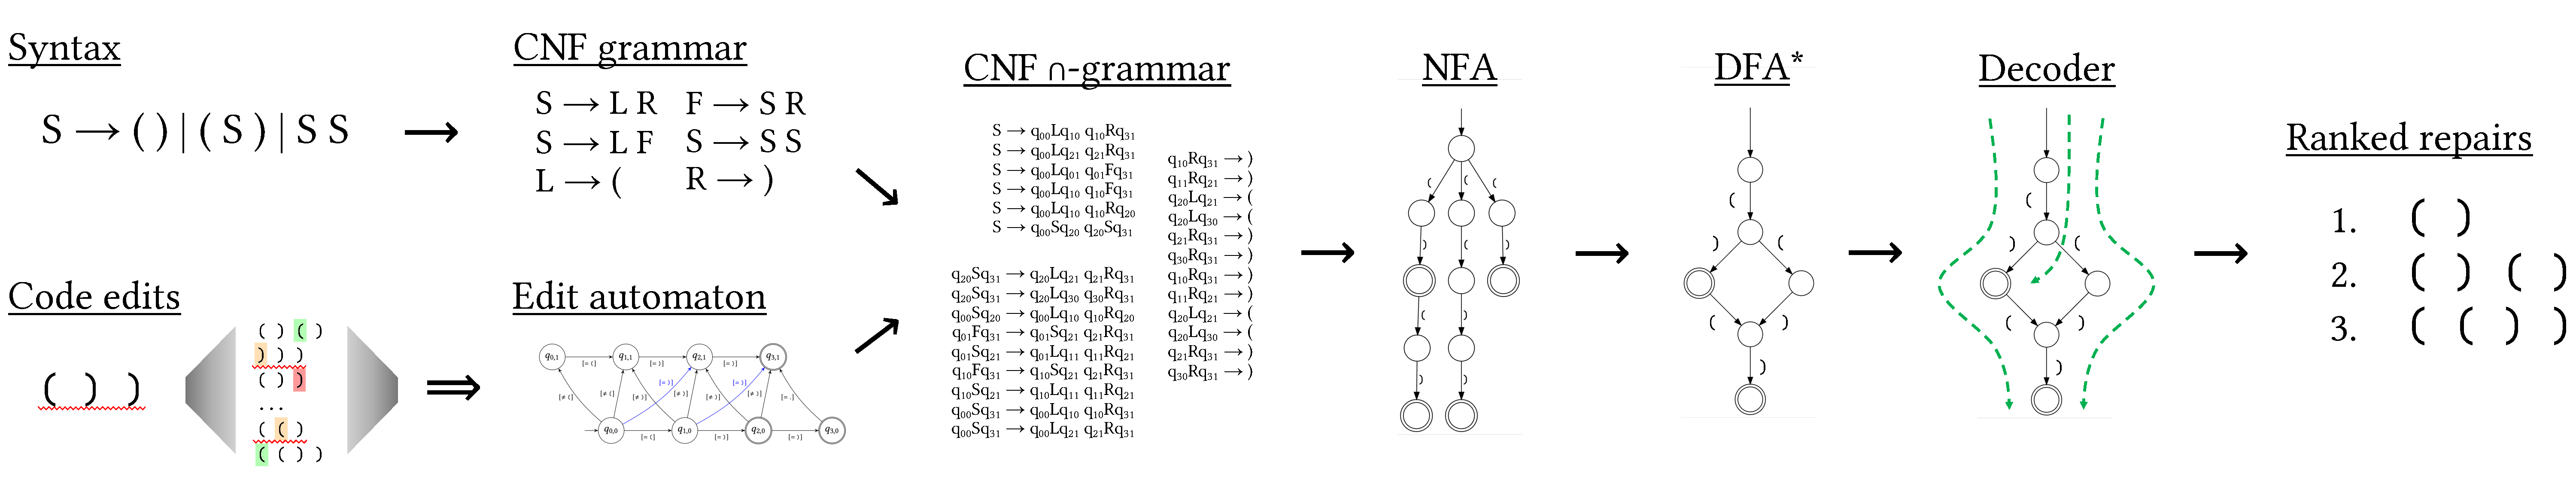
\includegraphics[width=\textwidth]{content/figures/flow.pdf}\vspace{-1pt}
  \caption{Simplified dataflow. Given a grammar and broken code fragment, we create an automaton generating the language of small edits, then construct a grammar representing the intersection of the two languages. This grammar can be converted to a finite automaton, determinized, then decoded to produce an explicit list of repairs.}\label{fig:arch_simp}
\end{figure}

The advantage of using this approach for syntax repair is that it performs the intersection not in the set domain, but in the domain of grammars and automata, thereby avoiding a great deal of useless work that would be necessary were we to compute the intersection by sampling and rejecting edits. Furthermore, it is a complete decision procedure, meaning that every possible repair within a given edit distance will eventually be found by the decoder.

To explain each component, we will require a more detailed background on the formal language theory, then we can describe the full Bar-Hillel construction and our specialization to Levenshtein automata intersections. But first, we will cover some related literature on program repair.

\clearpage